\documentclass[12pt]{jarticle}
\usepackage{TUSIReport}
\usepackage{otf}
\usepackage[dvipdfmx]{graphicx}
\usepackage[dvipdfmx]{color}
\usepackage{amsmath}
\usepackage{amssymb}
\usepackage{color}
\usepackage{hhline}
\usepackage{fancybox,ascmac}
\usepackage{multirow}
\usepackage{url}
\usepackage{bm}
\usepackage{listings,jlisting}

\begin{document}
%%%%%%%%%%%%%%%%%%%%%%%%%%%%%%%%%%%%%%%%%%%%%%%%%%%%%%%%%%%%%%
% 表紙を出力する場合は,\提出者と\共同実験者をいれる
% \提出者{科目名}{課題名}{提出年}{提出月}{提出日}{学籍番号}{氏名}
% \共同実験者{一人目}{二人目}{..}{..}{..}{..}{..}{八人目}
%%%%%%%%%%%%%%%%%%%%%%%%%%%%%%%%%%%%%%%%%%%%%%%%%%%%%%%%%%%%%%
\提出者{情報工学実験2}{実験テーマ5 教育システム設計}{2020}{11}{9}{4619055}{辰川力駆}
\共同実験者{}{}{}{}{}{}{}{}

%%%%%%%%%%%%%%%%%%%%%%%%%%%%%%%%%%%%%%%%%%%%%%%%%%%%%%%%%%%%%%
% 表紙を出力しない場合は,以下の「\表紙出力」をコメントアウトする
%%%%%%%%%%%%%%%%%%%%%%%%%%%%%%%%%%%%%%%%%%%%%%%%%%%%%%%%%%%%%%
\表紙出力

%%%%%%%%%%%%%%%%%%%%%%%%%%%%%%%%%%%%%%%%%%%%%%%%%%%%%%%%%%%%%%
% 以下はレポート本体である.別途 TeXファイルを作成し \input 使っても良い
%%%%%%%%%%%%%%%%%%%%%%%%%%%%%%%%%%%%%%%%%%%%%%%%%%%%%%%%%%%%%%

\section{要旨}
項目反応理論の紹介と、それを用いた場合の受験者の能力値の推定について学習し、
課題を通して演習を行う。

\section{目的}
統計モデルを用いた分析は、例えば商品の推薦や迷惑メールの削除機能など、
身近な機能を支える基本的な技術となっている。
本実験では、このような統計モデルを用いた分析に欠かせない、
パラメタの推定の方法について、
基本的な技術を習得することを目的とする。

\section{理論}
\subsection{項目反応理論基礎}
項目反応理論では、
ある受験者$j$がある項目$i$に正答する$x_{i,j}=1$確率を以下の式でモデル化する。
\begin{equation}
    P(x_{i,j}=1|\theta_j,a_i,b_i)=P_i(x_{i,j}=1|\theta_j)=P_i(\theta_j)=\frac{1}{1+\exp\{-Da_i(\theta_j -b_i)\}}
\end{equation}
ここで$\theta_j$は受験者の能力値パラメタ、
$a_i$は項目の識別力パラメタ、
$b_i$は項目の困難度パラメタである。
また、$D=1.7$としたとき、このモデルは以下の特徴がある。
\begin{enumerate}
    \item $\theta_j=b_i$の場合、正答確率は50$\%$となる。
    \item $\theta_j=b_i$での正答率の傾きは$a_i$に比例する。
    \item $a_i=1,b_i=0$のとき、この関数は累積標準正規分布の良い近似となる。
\end{enumerate}

$a$は識別力パラメタと呼ばれる。
$a$が0に近い項目は、
能力値によらず一定の正答率となるような、
能力に関係ない項目となる。
$a$が$0$に近い値の時は、能力値に関わらず正答率が高い傾向がある。

$b$は困難度パラメタと呼ばれる。
項目反応関数の正答確率が$50%$となる点の$\theta$と同じ値となる。
$b$が大きな項目では正答に必要な能力値が大きくなる。
$b$が大きいほど、小さい能力値での正答率が低い傾向がある。

\subsection{最尤推定を用いた受験者能力の推定}
項目反応理論を用いた受験者の能力値の推定も最尤推定と同様に計算する。
例えば、今ある問題に正答した$(x_{i,j}=1)$とする。
この時の受験者の能力値は以下の数式を考えれば良い。
\begin{equation}
    \hat{\theta}=\mathop{\rm arg~max}\limits_{\theta}P(\theta|x_{i,j}=1)
\end{equation}
ただし、
$P(\theta_j|x_{i,j}=1)$はIRTのモデルに従って直接は与えられていないため、
ベイズの定理より、$P_i(x_{i,j}=1|\theta_j)$を用いて考える。
\begin{eqnarray}
    P(\theta_j|x_{i,j}=1)=\frac{P(\theta_j)}{P(x_{i,j}=1)}P_i(x_{i,j}=1|\theta_j)
\end{eqnarray}
ここで、
$P(x_{i,j}=1)$はその問題に正答できる確率であるが、
変数$\theta_j$と独立な変数であるため、
$\mathop{\rm arg~max}\limits_{\theta}$を考える上で定数とみなすことができる。
従って、以下の式を考えても結果は変わらない。
\begin{eqnarray}
    \hat{\theta}&=&\mathop{\rm arg~max}\limits_{\theta}P(\theta|x_{i,j}=1) \\
    &=&\mathop{\rm arg~max}\limits_{\theta}P(\theta)P_i(x_{i,j}=1|\theta_j)
\end{eqnarray}
$P(\theta)$は能力値が一般にどのような分布をしているかを表すので、
標準正規分布していると仮定できる。
\begin{eqnarray}
    P(\theta)=\frac{1}{\sqrt{2\pi}}\exp \left(-\frac{\theta^2}{2}\right)
\end{eqnarray}
また、
誤答した場合も同様に以下のように考えることができる。
\begin{eqnarray}
    \hat{\theta} &=& \mathop{\rm arg~max}\limits_{\theta}P(\theta|x_{i,j}=0)\\
    &=& \mathop{\rm arg~max}\limits_{\theta}P(\theta)P_i(x_{i,j}=0|\theta_j)\\
    &=& \mathop{\rm arg~max}\limits_{\theta}P(\theta)(1- P_i(x_{i,j}=1|\theta_j))
\end{eqnarray}

このような関数を考えることで、
ある問題に正答、
あるいは誤答した場合の受験者の能力値を推定することが可能である。
また、$P(\theta)$は問題に正答したという事実を受け取る前の確率であり、
事前確率と呼ばれることがある。
加えて、$P(\theta|x_{i,j})$は問題に正答あるいは
誤答したという事実を受け取ったあとの確率なので、
事後確率と呼ばれることがある。

また、項目反応理論では、
項目情報量関数と呼ばれる指標が非常に重要となる。
項目情報量関数とは、
項目反応関数について項目への反応から能力値を推定する際のフィッシャー情報量を
算出したものであり、2パラメタロジスティックモデルでは以下のような式となる。
\begin{eqnarray}
    I_i(\theta)=D^2a_i^2 P_i(\theta)(1-P_i(\theta))
\end{eqnarray}
フィッシャー情報量は一般に$\hat{\theta}$の標準誤差${\rm se}(\hat{\theta})$
と以下の関係を持つ
\begin{eqnarray}
    {\rm se}(\hat{\theta})=I_i(\hat{\theta})^{-\frac{1}{2}}=\frac{1}{\sqrt{I_i(\hat{\theta})}}
\end{eqnarray}

そのため、この項目情報量を用いることで、
推定された$\hat{\theta}$に対してどの程度標準誤差があるかを見積もることができる。

\clearpage
\section{課題}
\subsection{課題2-1}
\begin{shadebox}
    課題1-3で解いた項目について、項目反応関数の概形を描く。
\end{shadebox}

課題1-3で解いた問題のパラメタについて表1にまとめた。
そして、それを基に項目反応関数の概形を描くと図1のようになった。
\begin{table}[htb]
    \begin{center}
        \caption{解いた問題の特性パラメタ}
        \begin{tabular}{|c|r|r|}
            \hline
            問題 & $aパラメタ$ & $bパラメタ$ \\
            \hline
            3    & 2.87168     & 0.69892     \\
            9    & 0.42082     & 0.22627     \\
            21   & 1.03497     & 0.31148     \\
            24   & 0.71798     & 1.22817     \\
            30   & 1.20718     & 0.65633     \\
            35   & 0.72641     & 0.14052     \\
            40   & 0.31796     & 2.23511     \\
            51   & 0.51611     & 0.94029     \\
            \hline
        \end{tabular}
    \end{center}
\end{table}
\begin{figure}[h]
    \begin{center}
        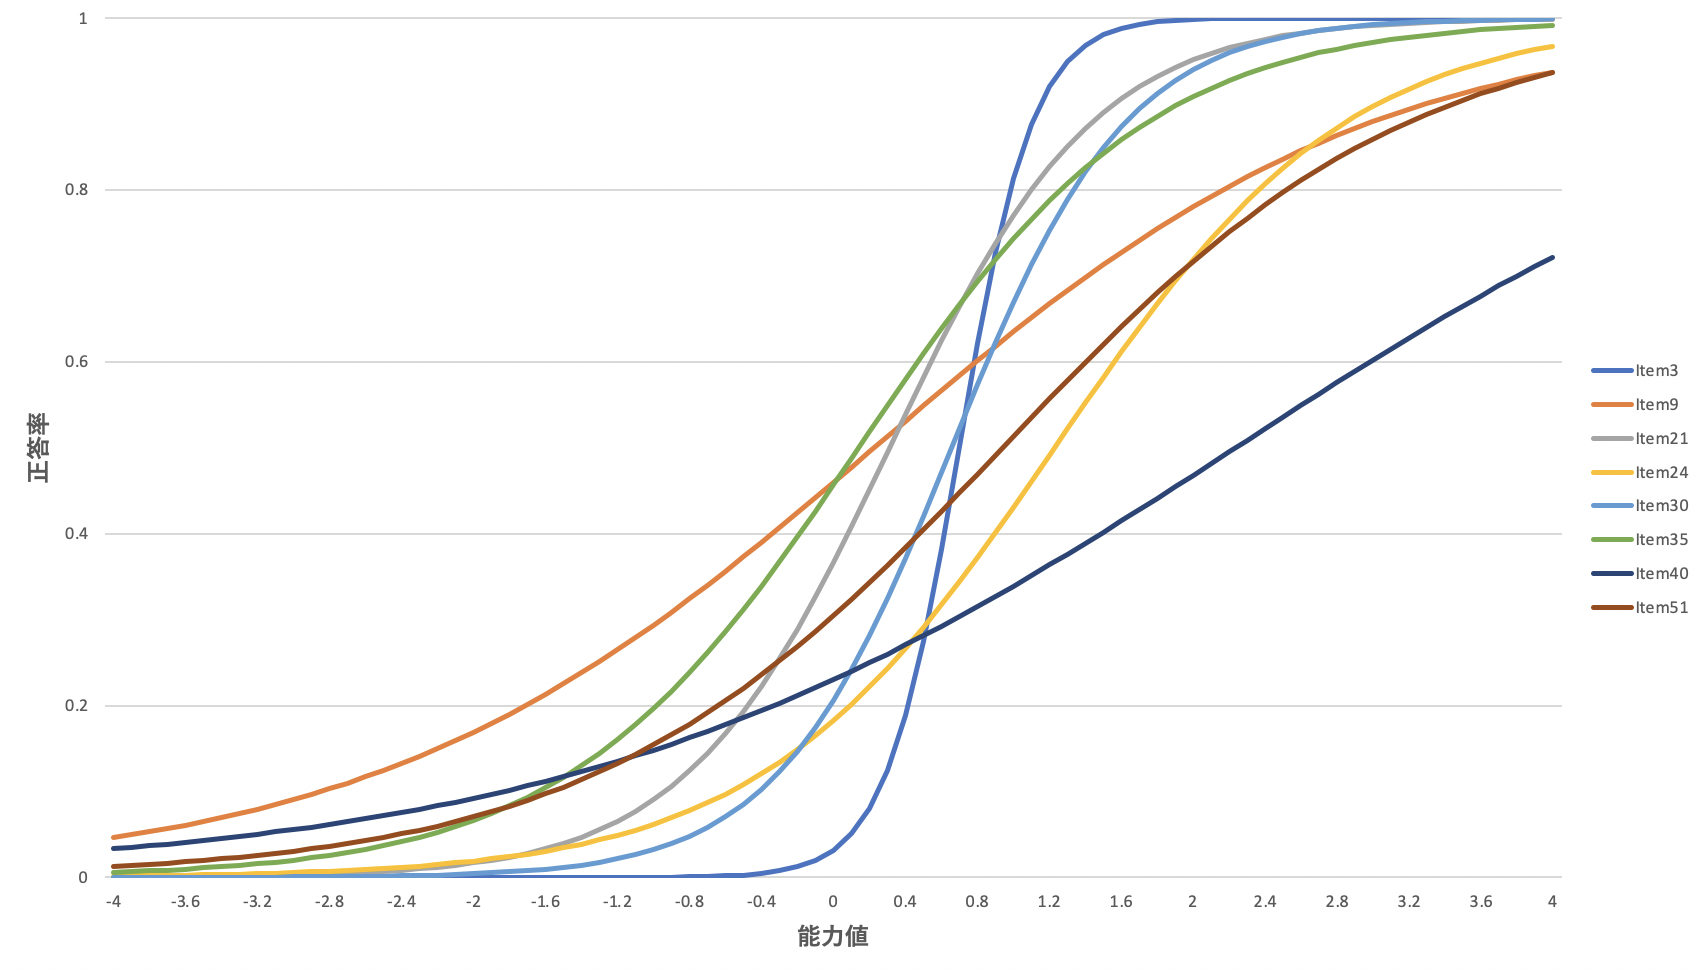
\includegraphics[scale=0.3]{kadai5_2_1.png}
    \end{center}
    \caption{項目反応関数}
\end{figure}

\clearpage
\subsection{課題2-2}
\begin{shadebox}
    課題2-1で描いたグラフを参考に、それらの項目がどのような項目であったのか考察する。
\end{shadebox}

図1のグラフの中央付近の増加量について、Item3が一番正答率の変化量が大きい。
これは、$a$パラメタが他と比べて大きいからである。
つまり、Item3などの$a$パラメタが大きい問題は、
ある一定の能力値を超えるとほぼ100%の正答率となるが、
逆にその能力値を越えていないとほぼ0%の正答率となることが分かる。

$b$パラメタについては、
Item40を見ると分かるように正答率が高くなるまでに必要な能力値が高いことがわかる。
つまり、$b$パラメタが低い順に正答率が50%になるための能力値が低い。

\subsection{課題2-3}
\begin{shadebox}
    $\theta_j=b_i$の場合、正答確率は$50%$であることを証明する。
\end{shadebox}

式(1)に$\theta_j=b_i$を代入して、
\begin{eqnarray*}
    P(\theta_j=b_i)&=&\frac{1}{1+\exp\{-Da_i(\theta_j -b_i)\}}\\
    &=&\frac{1}{1+\exp\{-Da_i(b_i -b_i)\}}\\
    &=&\frac{1}{1+\exp(0)}\\
    &=&\frac{1}{2}\\
    &=&0.5
\end{eqnarray*}
よって正答確率は$50%$となる。

\subsection{課題2c-1}
\begin{shadebox}
    $\theta_j=b_i$での項目反応関数の傾きは$a_i$に比例することを証明する。
\end{shadebox}

\clearpage
\subsection{課題2–4}
\begin{shadebox}
    課題1-3で解いた項目から1題選びその正誤から描かれる事後分布のグラフを示す。
\end{shadebox}

\subsection{課題2–5}
\begin{shadebox}
    課題2-4で描いた事後分布から能力値を推定する。
    またその時の標準誤差を求める。
\end{shadebox}
\subsection{課題2–6}
\begin{shadebox}
    ぱあ
\end{shadebox}
\subsection{課題2–7}
\begin{shadebox}
    ぱあ
\end{shadebox}

\section{まとめ}


% 参考文献
\begin{thebibliography}{99}
    \label{sannkoubunnkenn_chapter}
\end{thebibliography}

\clearpage
% 付録
\appendix
%%%%%%%%%%%%%%%%%%%%%%%%%%%%%%%%%%%%%%%%%%%%%%%%%%%%%%%%%%%%%%
\end{document}